
    \documentclass[tikz,convert={outfile=\jobname.png}]{standalone}
    \usetikzlibrary{mindmap,trees,backgrounds}
    \usepackage{fontspec}
    \defaultfontfeatures{Ligatures=TeX,Scale=3}
    \setmainfont{M+ 1mn}
    \begin{document}
    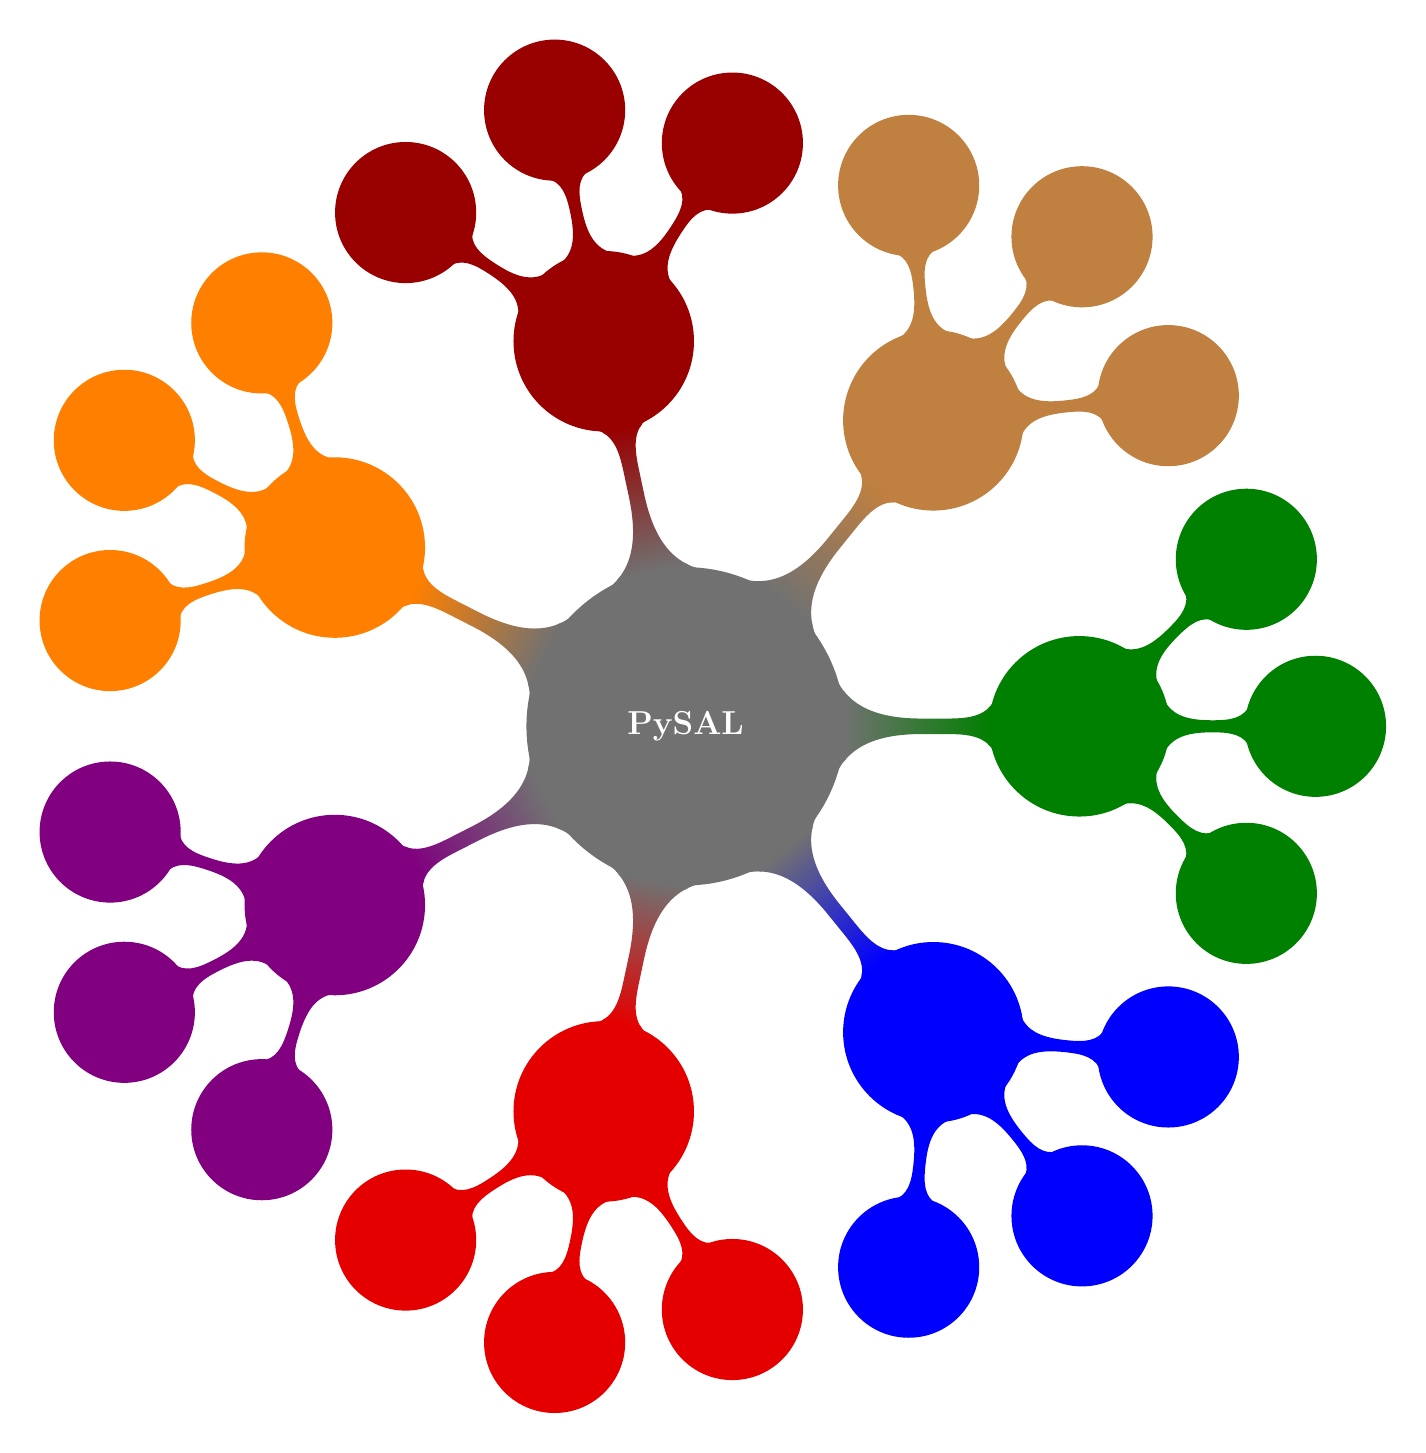
\begin{tikzpicture}[
        background rectangle/.style={fill=white},
        show background rectangle,
        mindmap,
        grow cyclic,
        every node/.style=concept,
        concept color={rgb:black,1.25;white,1},
        text=white,
        level 1/.append style={
            level distance=5cm,
            sibling angle=51,
            font=\Huge
        },
        level 2/.append style={
            level distance=3cm,
            sibling angle=45
        }
    ]
    
        \node[concept color={rgb:black,1.25;white,1}]{\large\bfseries{PySAL}}
        child [concept color=violet]{ node {}
            child { node { }}
            child { node { }}
            child { node { }}
         }
        child [concept color=black!10!red]{ node {}
            child { node { }}
            child { node { }}
            child { node { }}
         }
        child [concept color=blue]{ node {}
            child { node { }}
            child { node { }}
            child { node { }}
         }
        child [concept color=black!50!green]{ node {}
            child { node { }}
            child { node { }}
            child { node { }}
         }
        child [concept color=brown]{ node {}
            child { node { }}
            child { node { }}
            child { node { }}
         }
        child [concept color=black!40!red]{ node {}
            child { node { }}
            child { node { }}
            child { node { }}
         }
        child [concept color=orange]{ node {}
            child { node { }}
            child { node { }}
            child { node { }}
         }
                ;
    \end{tikzpicture}
    \end{document}